
\section{Dependency Rule Synthesis}
\label{s:algorithm}

\todo{intro}

% TODO Type setting: make R --> mathcal{R} b/c it's a set of rules
This section outlines the algorithm \depsynth uses to solve the dependency rule
synthesis problem for a storage system.
First, we show the top-level algorithm of \depsynth, which generates rules
for a set of litmus tests using two subroutines.
Next, we describe the algorithm for finding a set of rules for a single litmus test.
We also define the language for generated rules in this part.
Finally, we describe the subroutine for resolving conflicts between the rules
generated for single litmus tests.

\subsection{Problem Statement}

The crash consistency synthesis problem
that \depsynth solves
is to find a \emph{single} set of dependency rules $R$
that makes every litmus test $T$
in a set of tests $\mathcal{T}$
crash consistent (\cref{def:crash-consistent}).
As \cref{sec:problem:tests} discusses,
the set of tests $\mathcal{T}$ of interest
can be drawn from a number of sources,
including hand-written tests
and automated fuzzing or enumeration.

While \cref{def:crash-consistent} suffices to find a set of rules $R$
that guarantees crash consistency,
it does not rule out vacuous solutions that cannot be executed on real hardware.
For example, consider a program $P$
where $\interpret{P} = [\texttt{write}(a_1, v_1, \langle n_1, t_1 \rangle), \texttt{write}(a_2, v_2, \langle n_2, t_2 \rangle)]$.
The set of rules $R = \{ \deprule{n_1}{n_2}{=}, \deprule{n_2}{n_1}{=} \}$
makes this program crash consistent.
But this is a vacuous solution---%
the rules do not admit any valid crash schedules
other than the trivial $\vec{s} = \vec{\top}$ and $\vec{s} = \vec{\bot}$ schedules,
as \cref{def:valid-schedule} forces $s_1 = s_2$.
In effect, crash consistency for this program
requires both writes to happen ``at the same time'',
but on real disks the level of write atomicity is only a single data block,
so there is no way for both writes to happen at the same time.
To rule out such vacuous solutions,
we follow the example of happens-before graphs~\cite{lamport:happens-before}
from distributed systems and memory consistency,
and require the set of synthesized dependency rules $R$ to be \emph{acyclic}.

\subsection{Top-Level Algorithm}
In this section, we discuss the top-level algorithm of \depsynth, which iteratively
constructs a set of rules that satisfies all input litmus tests. \depsynth solves the
dependency rule synthesis problem in a per-litmus-test way, solving the sub-problem of
of synthesis for rules over single litmus tests in the input set before combining their
results.
Intuitively, solving our problem incrementally allows \depsynth to gradually build
up a set of rules, allowing it to synthesize a relatively small number of
rules at each step.
This is more scalable than synthesizing all rules at once, since
the rules search is super-polynomial in the number of disk writes considered.
% TODO is this second-to-last sentence necessary?
The sub-routine for solving the dependency rule synthesis problem over single tests,
\rulessearch, is described in \autoref{s:rulessearch}.


As \depsynth iteratively solves the problem for single tests, it may encounter a conflict
between the solutions for different tests.
Specifically, we say that some sets of rules contains a conflict when the rule sets
themselves are acyclic, but unioning the rules together introduces a possible cycle.
With this happens, \depsynth resolves the conflict
by searching for a set of rules that solves the rule synthesis problem for all litmus tests involved
in the conflict. The sub-routine for resolving conflicts, \resolvecons, is described in
\autoref{s:resolvecons}.

Previously, we have described rules as outputting a set of propositional logic constraints
over boolean variables that pertain to buffered disk writes.
To better explain the design and intuition behind \depsynth in this section,
we will often think of the output of rules instead as a \textit{dependency graph} over
writes. An edge in such a graph specifies a ``happens before'' relationship,
so an edge, or \textit{dependency}, from $w_0$ to $w_1$
(written $\depedge{w_0}{w_1}$) corresponds directly to
the constraint $\syncbool_0 \implies \syncbool_1$ over schedules for
writes including $w_0$ and $w_1$.

There are three requirements on the output rules of \depsynth.
The first two are described in \autoref{def:rule-synth-problem}: any rules output by \depsynth
must both be \textit{sufficient} (i.e. guarantee that any valid execution of any input litmus test
results in a crash consistent disk state)
and \textit{acyclic} (i.e. rules should not generate cyclic constraints on the schedule).
Our third constraint has to do with the efficiency of the output rules.
Rules that are both sufficient and acyclic may still introduce unnecessary constraints
on schedules over writes from a litmus test.
For example, take the litmus test
\begin{align*}
  &\putreq\ A\ 1\\
  &\putreq\ B\ 2
\end{align*}
which generates writes $w_{ai}, w_{ad}, w_{bi}, w_{bd}$ for the index and data writes
for the first and second put respectively.
A set of rules may create dependencies
$\depedge{w_{ai}}{w_{ad}}, \depedge{w_{ad}}{w_{bi}}, \depedge{w_{bi}}{w_{bd}}$
while only the first and last are necessary.
Additional constraints on valid schedules such as the one from this example can worsen
efficiency, as the disk has fewer schedules to choose from when committing writes.
Depending on the disk hardware, some schedules are more efficient than others \todo{cite},
so the output of \depsynth should restrict schedules as little as possible.
To prevent frivolous constraints, we require the output of \depsynth to be
\textit{minimal}. Rules are minimal whenever removing a single rule from the set
causes the set to no longer satisfy \autoref{def:rule-synth-problem}.

In some cases, it is not possible to generate a set of rules that solves our
synthesis problem. For example, if we take the example store from \autoref{s:overview}
with crash consistency property $\bot$, then no set of rules is sufficient.
When this is the case, \depsynth returns $\bot$ to indicate that it cannot find
a set of rules that satisfies our synthesis problem. Note that since \depsynth
is complete, this only occurs when no sufficient, acyclic set of rules exists.

\autoref{alg:top-level} gives the top-level algorithm of \depsynth.
For each litmus test in the input set, \toplevel first finds a set
of rules that satisfies the dependency rule synthesis problem over
that single test using \rulessearch. It stores these rules in a map $\Pi$
from tests to rules so that the set of tests causing a conflict in the
rules can easily be determined. Consider $\cup\Pi$ to be the union of all rules
in the map $\Pi$. We say that rules $\cup\Pi$ have
a conflict when it is \textit{not} acyclic. This is considered a conflict because the output
of \rulessearch is guaranteed to be acyclic, so $\cup\Pi$ can only be acyclic
when rules from multiple litmus tests combine to make a cycle.
\toplevel determines if a set of rules has a conflict (and which rules are involved in the conflict)
with \textproc{ConflictingTests}, which implements the check for acyclicity described in \autoref{s:problem}.
When this happens, \toplevel performs conflict resolution for the conflicting
tests and updates the dependency rules for each test accordingly.
Once this loop has completed, \toplevel outputs $\cup\Pi$.

\begin{figure}[h]
\begin{algorithmic}[1]
  \Function{DepSynth}
    {$\mathcal{L}, \mathcal{P}$} \Comment{Set of Litmus Tests, Crash Consistency Property}
    \State $\Pi \gets \{\}$ \Comment{Map from litmus tests to rules, $\cup\Pi$ is all rules}
    \For{$L\in\mathcal{L}$}
      \State $R \gets \Call{RulesSearch}{L, \mathcal{P}}$
      \If{$R = \bot$}
        \State \Return $\bot$
      \EndIf
      \State $\Pi \gets \Pi[L \mapsto R]$
      \State $\xi \gets \Call{ConflictingTests}{\Pi}$
        \Comment{Set of tests that cause conflict in $\cup\Pi$}
      \If{$\xi \neq \emptyset$}
        \State $\Theta \gets \Call{ResolveConflicts}{\xi,\Pi(\xi)}$
        \If{$\Theta = \bot$}
          \State \Return $\bot$
        \EndIf
        \For{$(L, R')\in\Theta$}
          \State $\Pi \gets \Pi[L \mapsto R']$
        \EndFor
      \EndIf
    \EndFor
    \State \Return $\cup\Pi$
  \EndFunction
\end{algorithmic}
\caption{Algorithm used by \depsynth to find a set of rules for all litmus tests.\tighten}
\label{alg:top-level}
\end{figure}

\subsection{Searching for Dependency Rules}
\label{l:rulessearch}
In this section, we describe our algorithm for finding rules for a single
litmus test. We break this search into two parts:
First, find a set of dependencies over the writes generated by the test
such that all valid schedules w.r.t. the dependencies result in
a crash consistent disk state.
Next, convert the set of dependencies into a set of rules.
As discussed previously, we call a set of dependencies
a dependency graph, where each write represents a node in the graph.
Like dependency rules, the dependency graph for any litmus test should satisfy
three properties:
\begin{enumerate}
  \item The graph is \textit{sufficient}, meaning that executing any schedule
        of writes that adheres to the graph will result
        in a disk state that satisfies the crash consistency property.
  \item The graph is acyclic
  \item The graph is \textit{minimal}, meaning that there is no subgraph
        that also satisfies the previous two properties
\end{enumerate}
These properties are necessary to allow \depsynth to convert dependency graphs
from \rulessearch into sufficient, acyclic, minimal sets of rules.

We first describe the design of our depenency graph
search algorithm, starting from a basic solution and
gradually increasing the complexity by applying optimizations. We argue that
the basic algorithm satisfies these three objectives and that the optimizations
preserve the correctness of the base algorithm.
After this, we describe the language for dependency rules and show how to generate rules
from a dependency graph.

\subsubsection{Dependency Graph Search}
% There are three levels of complexity to the dependency graph search algorithm:
% (1) Depth-first search, removing single edges, checking feasibility at each stage
%     and possibly backtracking
\paragraph{Removing Edges from a Complete Graph}
For our base algorithm, we take a top-down approach, starting from a complete graph
over the writes from a litmus test and gradually removing edges until we arrive
at a sufficient, acyclic graph. Compared to starting from an empty graph and
gradually adding edges, our top-down approach allows \depsynth to more easily
determine if a branch of the search is feasible or not, allowing for pruning.
For now though, we discuss the edge removal algorithm in the absence of pruning
so that we can more easily show the design and corretness of our final algorithm.

Our edge removal algorithm works as follows.
Start with a complete graph over the set of writes $\omega$. From this, we gradually remove
edges one at a time. To see if we should return a graph $\Gamma$, we first check
if we could return a smaller graph $\Gamma - \{\gamma\}$. If not, and if
$\Gamma$ is both sufficient and acylic, then we return $\Gamma$. Otherwise,
we return $\bot$ to mean that no subgraph of $\Gamma$ satisfies all three objectives.
The sub-procedure \graphsuff checks graph sufficiency with test $L$, property $\mathcal{P}$,
and transition function $f$ as follows:
\begin{enumerate}
  \item Convert the graph into a set of rules $R$.
  \item Using an SMT query, determine
    $\exists d.\exists S.\  
       f((d,\{\}), L) = (d', W)
       \wedge \valid(S,W,R)
       \wedge \neg\mathcal{P}(\crash(d',S,W), L)$
       with validity function $\valid$ and crash function $\crash$ as defined in \autoref{s:problem}.
       The starting graph is sufficient iff the query is \texttt{unsat}.
\end{enumerate}
Our edge removal algorithm is desicribed in \autoref{alg:remove-edges}.

%We can also add a pruning function \prune to this algorithm. For now, we will discuss
%this base algorithm with a \prune function that always returns \false, meaning
%that no graphs are pruned. Later in this section, we will show how to define a useful
%pruning function and show that it preserves soundness and completeness.

%If no remaining edges can be
%removed while preserving this objective \textit{and} there are no cycles in the graph,
%the algorithm has reached a minimal graph, so it returns the graph. Otherwise,
%if the graph is not acyclic and still cannot remove edges preserving (1),
%the algorithm backtracks to a previous state and then chooses a different edge to
%remove. If no graph exists that satisfies all three properties, then the algorithm
%outputs $\bot$.

\begin{figure}[h]
\begin{algorithmic}[1]
  \Function{GraphSearch}
    {$L, \mathcal{P}$} \Comment{Litmus test, Crash Consistency Property}
    \State $\omega \gets \Call{Writes}{L}$ \Comment{Set of all writes}
    \State $\Gamma \gets \omega \times \omega$ \Comment{Set of all possible dependency edges, making a complete dependency graph}
    \State \Return \Call{GraphSearchHelper}{$L,\mathcal{P},\Gamma$}
  \EndFunction

  \Function{GraphSearchHelper}
    {$L, \mathcal{P}, \Gamma$} \Comment{Litmus test, Crash Consistency Property, Candidate Dependency Graph}
    \For{$\gamma\in\Gamma$}
      \State $\Gamma' \gets \Call{GraphSearchHelper}{L, \mathcal{P}, \Gamma - \{\gamma\}}$
      \If{$\Gamma' \neq \bot$}
        \State \Return $\Gamma'$
      \EndIf
    \EndFor
    \If{$\graphsuff(L, \mathcal{P}, \Gamma) \wedge \acyclic(\Gamma)$}
      \State \Return $\Gamma$
    \EndIf
    \State \Return $\bot$
  \EndFunction
\end{algorithmic}
\caption{Algorithm for finding a dependency graph given a litmus test and a crash consistency
property; based on removing edges and backtracking.\tighten}
\label{alg:remove-edges}
\end{figure}

To better understand our edge removal algorithm, again consider the example
litmus test $ \putreq\ A\ 1;\ \putreq\ B\ 2$
which generates writes $w_{ai}, w_{ad}, w_{bi}, w_{bd}$.
The smallest sufficient dependency graph for this example contains two edges:
$\depedge{w_{ai}}{w_{ad}}$ and $\depedge{w_{bi}}{w_{bd}}$.
\autoref{fig:basic-search-visual} shows the search tree for this example,
illustrating how \graphsearch realizes this dependency graph.

We now argue that the algorithm shown in \autoref{alg:remove-edges} is both sound and complete, meaning that
\begin{enumerate}[(a)]
\item Any dependency graph output by \graphsearch is a minimal, acyclic graph such that executing
      and schedule of writes that is valid w.r.t. the output graph and writes $\getwrites(L)$
      results in a crash consistent disk state (i.e. soundness).
\item If there exists such a dependency graph that satisfies these properties (i.e. sufficient, minimal,
      acyclic), then \graphsearch will output some graph that satisfies the properties.
\end{enumerate}

To show why \graphsearch is sound, we need to show that any non-$\bot$ output satisfies the three
objectives previously described: (1) executing any schedule allowed by the graph results in a crash
consistent disk state, (2) the graph is acylic, and (3) the graph is minimal. For (1) and (2), notice
that any non-$\bot$ $\Gamma$ returned is either returned in a branch guarded by checks
for sufficiency acyclicity or returned from a recursive call. For (3), notice that $\Gamma$ is only returned
when there is no smaller graph $\Gamma - \{\gamma\}$ that is sufficient and acylic.
This means that any $\Gamma$ returned at the end of the first branch (and thus any non-$\bot$ $\Gamma$ returned)
must be minimal.

We can show that \graphsearch is complete by proving the contrapositive: when \graphsearch outputs $\bot$,
there is no dependency graph that is sufficient, minimal, and acyclic. For all graphs $\Gamma$ enumerated
by \graphsearch, it must be the case that all subgraphs $\Gamma'\subset\Gamma$
are not both sufficient and acylic \textit{and} that $\Gamma$ itself is not both sufficient and acylic
(otherwise, \graphsearch would return either some $\Gamma'$ or $\Gamma$). Since \graphsearch enumerates
all subgraphs $\Gamma\subset\omega\times\omega$, there must be no sufficient, acyclic, minimal dependency graph.
Thus \graphsearch is complete.

\begin{figure}
  \centering
  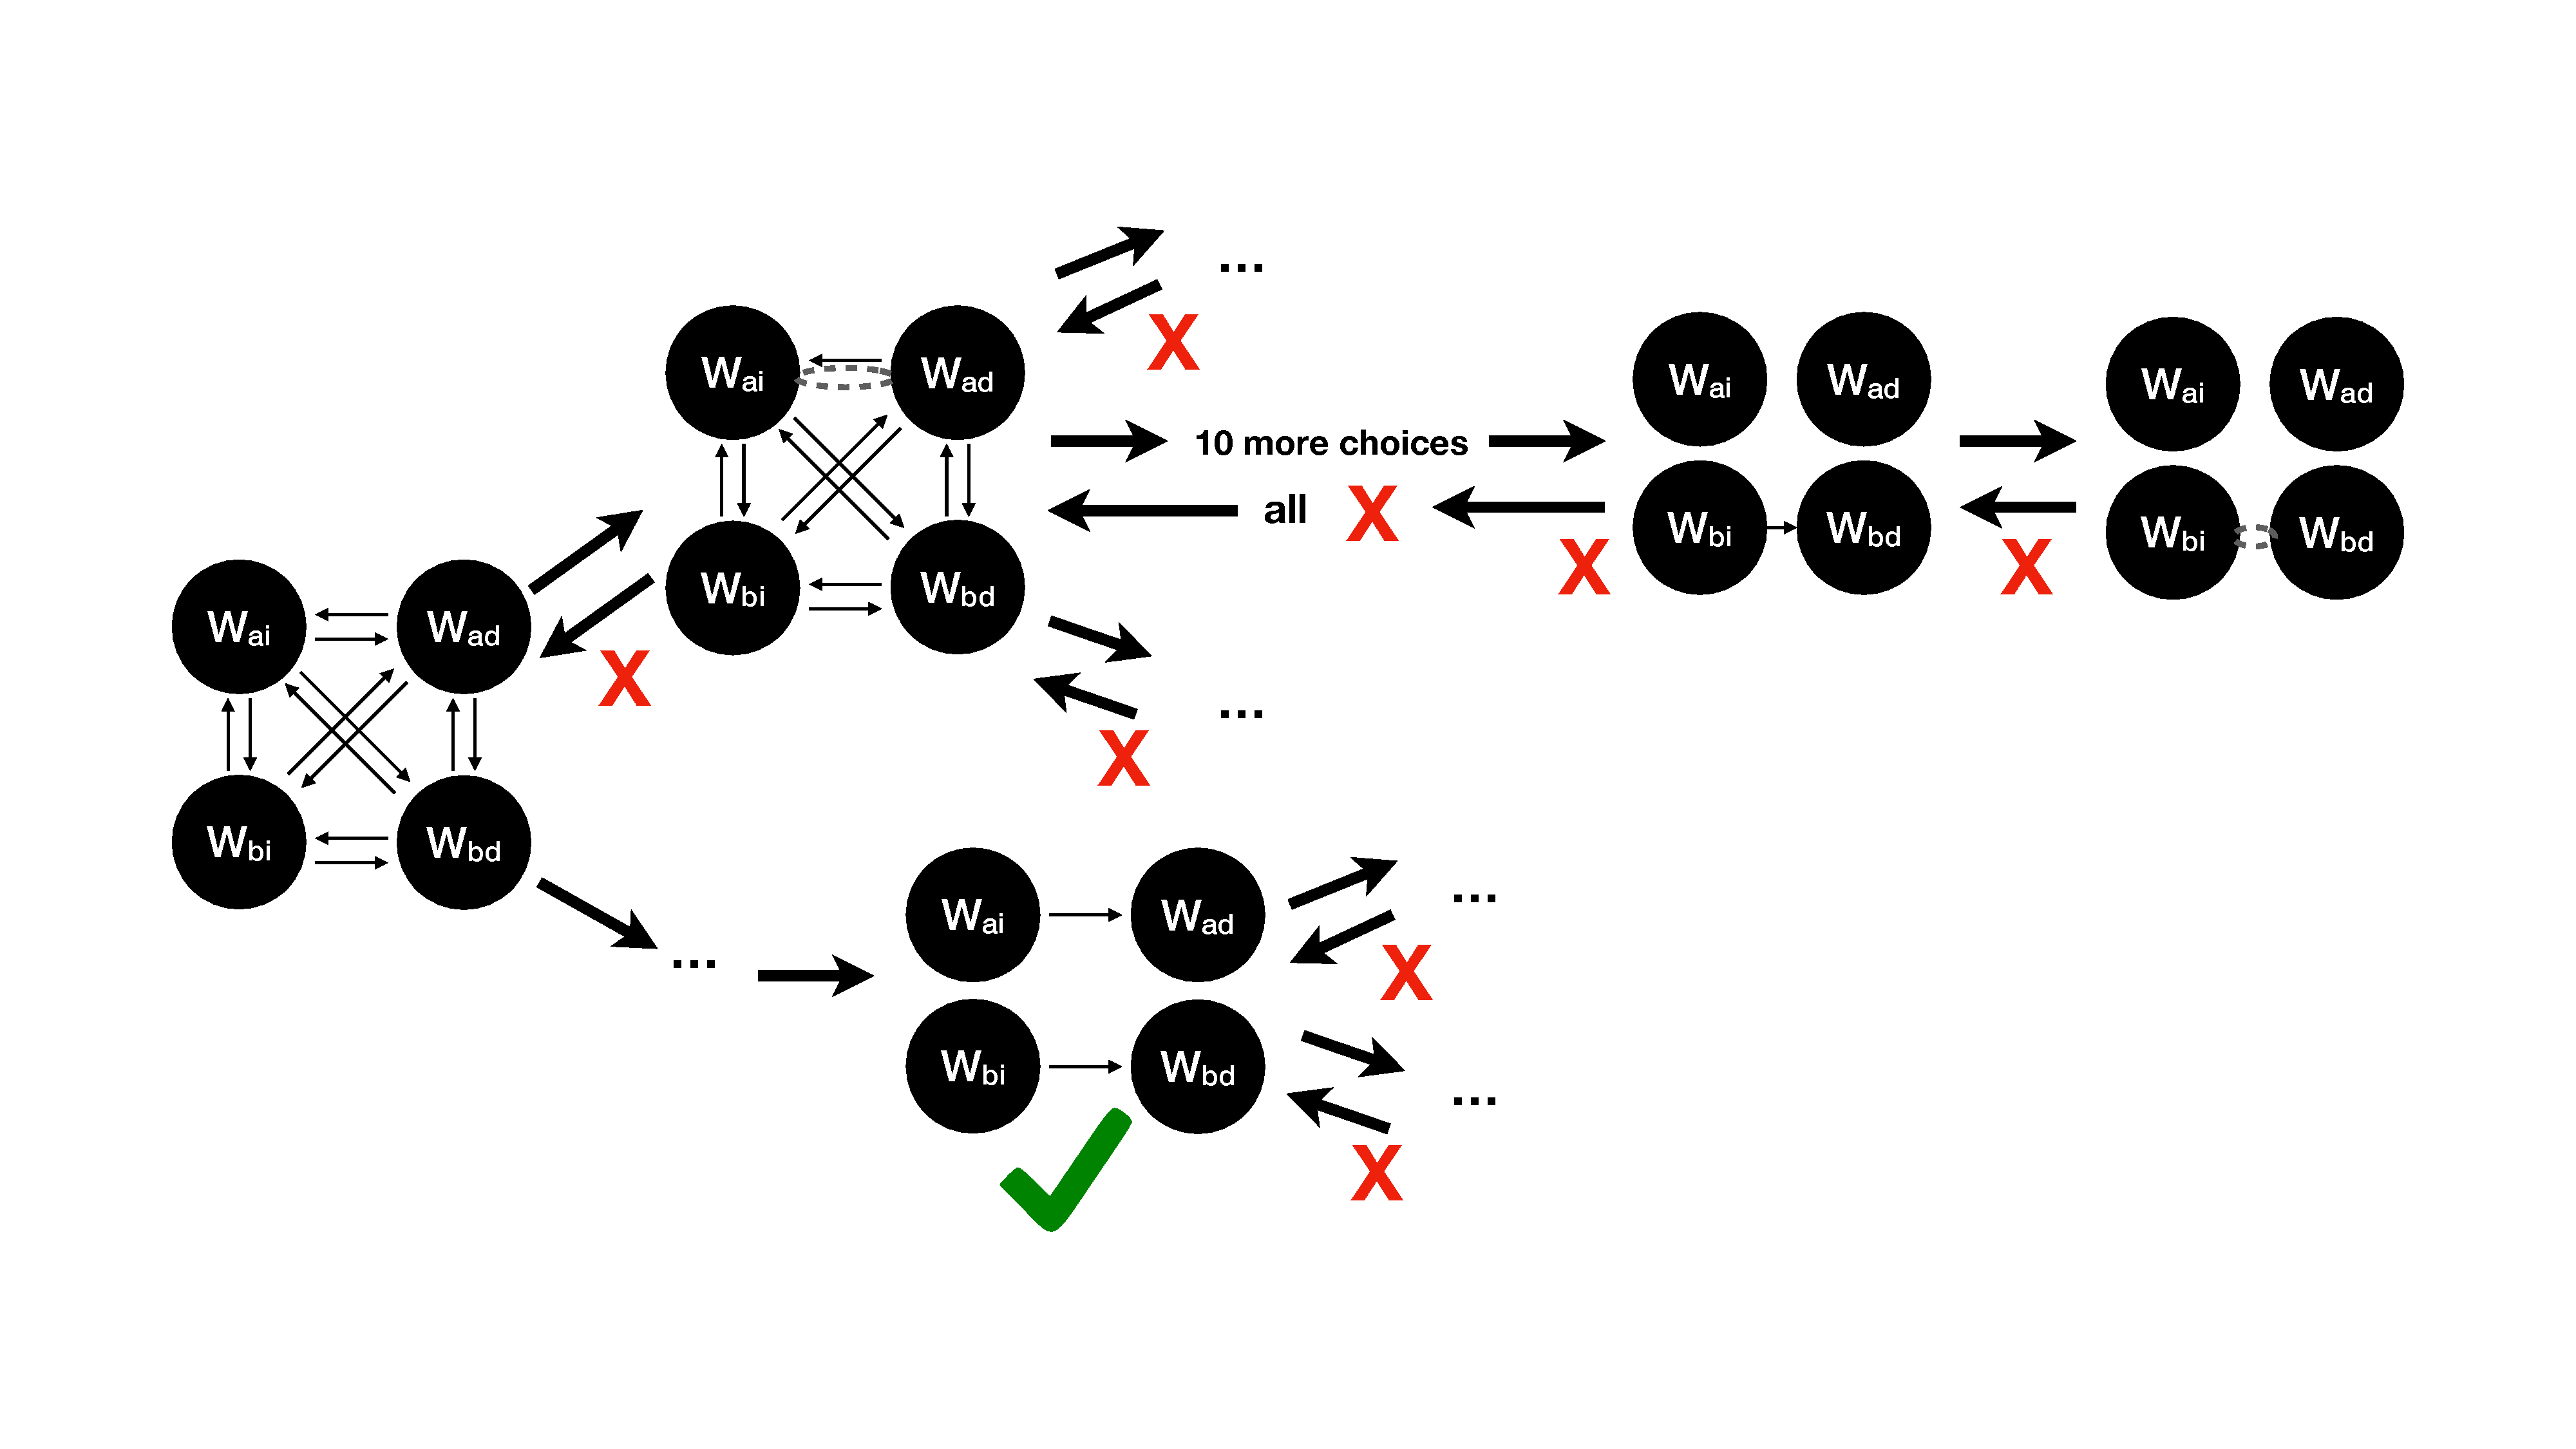
\includegraphics[clip,trim=0cm 5cm 0cm 5cm,width=0.9\linewidth,page=1]{graph-search-graphics.pdf}
  \caption{The search tree for a dependency graph over writes from litmus test
           $ \putreq\ A\ 1;\ \putreq\ B\ 2$ using
           the basic dependency graph search algorithm: \graphsearch.
           Candidates are shown traversed left-to-right, top-to-bottom.
           Starting with a complete graph, the search branches by choosing a single edge to remove.
           When \graphsearch finds a graph that is sufficient, acyclic, and where none of its children
           are sufficient, the algorithm returns.\tighten}
  \label{fig:basic-search-visual}
\end{figure}

% (2) Optimizing search by making multiple decisions at once. Two ways to think about
%     this: (a) remove multiple edges at once or (b) splitting SCCs
%     Both are viable choices, went with (b) because backtracking tends to work better
%     (and it also lends itself better to heuristics/learning)
%     In fact, (b) can be viewed as a specific form of (a).
%     We split SCCs one _write_ at a time, by which we mean when splitting SCC (x y z ...),
%     we pick one write (say x) to remove and either order the SCC (x) before or after SCC
%     (y z ...). "Order before/after" simply means removing all edges (_ x) or (x _) respectively.
\paragraph{Searching with SCCs}
The algorithm shown in \autoref{alg:remove-edges} starts from a complete dependency graph and removes single
edges (while possibly backtracking) to achieve a sufficient, acyclic, minimal graph. While this strategy
is sound and complete, removing edges one-by-one results in long search paths that make backtracking slow.
Specifically, if a bad choice is made early in the search, \autoref{alg:remove-edges} may spend a long time
searching in a subspace with no solution. Moreover, multiple branches in the search may lead to the same graph
(by removing the same edges in a different order), so there is headway to improve our search
with partial order reduction.

One observation that allows us to more efficiently explore the search space is that,
because of the requirement on dependency graphs to be acyclic, it suffices to first
find a total order over all nodes, then find a minimal graph whose edges go in the
direction of that order. By gradually building up an order, we can avoid considering
as many intermediate states as our basic edge removal algorithm.
Doing so allows for more efficient backtracking: with fewer intermediate states,
fewer choices must be reversed when a branch of the search is found to be infeasible.
The tradeoff here is that exploring an infeasible branch is more likely,
as each decision eliminates a larger portion of the search space.
For this reason, \autoref{s:impl} describes how to avoid infeasible branches
as much as possible using knowledge of our domain.

\depsynth implements the search for a total order over nodes
by restructuring our search into one over \textit{orderings of
strongly connected components} in the graph. A strongly connected component (SCC) in graph $\Gamma$ is a subset of
writes $W\subset \omega$ such that for all pairs $w_i,w_j$ in $W$, there exists some path from $w_i$ to $w_j$
in $\Gamma$. The goal of our new search is to find a total order over the writes $\omega$ (which is represented
by a DAG $\Gamma$), then reduce the total order to a minimal graph by greedily removing edges.
We do this by gradually splitting SCCs in $\Gamma$ and ordering the newly formed SCCs.

Similar to \autoref{alg:remove-edges}, we start with a complete graph, so there is one SCC: $\omega$.
Then, at each stage of our new algorithm, we choose one write to decouple from its strongly connected component,
either ordering it before or after the other nodes in the SCC. To do so, we remove all edges that conflict
with the decided ordering from $\Gamma$. Eventually, the algorithm reaches a graph will only singleton SCCs,
at which point it uses \autoref{alg:remove-edges} to return either a minimal graph or $\bot$ if no subgraph
is sufficient. This improves upon our base algorithm because instead of (at most) $n(n-1)$
choices at each decision and paths to a solution of length (at most) $n(n-1)$, our new algorithm has (at most) $2n$
decisions and solution paths of length (at most) $n$. This algorithm is shown in \autoref{alg:scc-search}.
Note that since any $\Gamma'$ passed to $\textproc{GraphSearchHelper}$ are always
sufficient and acylic, $\textproc{GraphSearchHelper}$ acts as a greedy edge-removal procedure.

\begin{figure}[h]
\begin{algorithmic}[1]
  \Function{SccGraphSearch}
    {$L, \mathcal{P}$} \Comment{Litmus test, Crash Consistency Property}
    \State $\omega \gets \Call{Writes}{L}$ \Comment{Set of all writes}
    \State $\Gamma \gets \omega \times \omega$ \Comment{Set of all possible dependency edges, making a complete dependency graph}
    % \State $\mathcal{C} \gets \{\omega\}$ \Comment{Starting SCCs is the singleton containing $\omega$}
    \State \Return \Call{SccGraphSearchHelper}{$L,\mathcal{P},\Gamma$}
  \EndFunction

  \Function{SccGraphSearchHelper}
    %{$L, \mathcal{P}, \Gamma, \mathcal{C}$} \Comment{Litmus test, Crash Consistency Property,
    %                                                 Candidate Dependency Graph, Set of SCCs}
    {$L, \mathcal{P}, \Gamma$} \Comment{Litmus test, Crash Consistency Property, Candidate Dependency Graph}
    \State $\Theta \gets \Call{GetSCCs}{\Gamma}$
    \If{$\forall \theta\in \Theta. |\theta| = 1$}
      \State \Return \Call{GraphSearchHelper}{$L,\mathcal{P},\Gamma'$}
    \EndIf
    \If{$\neg\graphsuff(L, \mathcal{P}, \Gamma)$}
        \Comment{If $\Gamma$ is not sufficient, no subgraphs of $\Gamma$ are sufficient}
      \State \Return $\bot$
    \EndIf
    \For{$\theta\in\Theta$}
      \For{$w\in \theta$}
        \State $\Gamma_r \gets \Call{SccGraphSearchHelper}{L, \mathcal{P}, \Gamma - \{(w, w_i) | w_i \in \theta\}}$
        \If{$\Gamma_r \neq \bot$}
          \State \Return $\Gamma_r$
        \EndIf
        \State $\Gamma_l \gets \Call{SccGraphSearchHelper}{L, \mathcal{P}, \Gamma - \{(w_i, w) | w_i \in \theta\}}$
        \If{$\Gamma_l \neq \bot$}
          \State \Return $\Gamma_l$
        \EndIf
      \EndFor
    \EndFor
    \State \Return $\bot$ \Comment{Cannot remove edges to make $\Gamma$ acyclic}
  \EndFunction
\end{algorithmic}
\caption{Algorithm for finding a dependency graph given a litmus test and a crash consistency
property; based on finding a total order over the nodes and then greedily removing edges.\tighten}
\label{alg:scc-search}
\end{figure}

We illustrate concretely the benefits of an SCC-based search
over an edge removal search by using our same example
litmus test $ \putreq\ A\ 1;\ \putreq\ B\ 2$ from earlier.
In \graphsearch, removing the edge $(w_{ai},w_{ad})$
results in exploring a large, infeasible search space
of graphs without $(w_{ai},w_{ad})$.
\graphsearch eventually discovers that this branch is infeasible,
but not until individually checking the sufficiency and acyclicity
of each subgraph.
When \sccsearch makes a similarly wrong decision --- ordering $w_{ai}$
after other nodes --- it can escape the infeasible branch much more quickly,
as there are much fewer candidates to check.
\autoref{fig:scc-search-visual} shows the search tree using \sccsearch for this example.

\autoref{alg:scc-search} also introduces pruning on top of the base algorithm from \autoref{alg:remove-edges}.
Specifically, we make the observation that if a graph $\Gamma$ is not sufficient for a litmus test
and crash consistency property, then no subgraph of $\Gamma$ is sufficient for such a test and property.
Using this, \sccsearch prunes branches of the search where the parent graph is not sufficient.

Before moving on, we argue that these optimizations on top of our base algorithm from \autoref{alg:remove-edges}
maintains correctness (i.e. both soundness and completeness). We first argue the correctness of \sccsearch
without pruning, then show the correctness of our pruning technique.

Starting with soundness, notice that like \autoref{alg:remove-edges},
\textproc{SccGraphSearchHelper} only returns non-$\bot$ $\Gamma'$ guarded by a check for sufficiency.
Additionally, non-$\bot$ $\Gamma'$ is only returned when all SCCs have size $1$, meaning that there cannot be
cycles in $\Gamma'$. Finally, to achieve minimality, edges are greedily removed from $\Gamma'$ by
\textproc{GraphSearchHelper}, which we've previously shown to return minimal graphs.

Now we show that \autoref{alg:scc-search} presents a complete algorithm. To do so, we show that any graph
returned by \autoref{alg:remove-edges} can be reached by \autoref{alg:scc-search}. Consider a sufficient, acyclic,
minimal graph $\Gamma$ returned by \autoref{alg:remove-edges}. Add edges to $\Gamma$ to make a total order over all
writes, and call this new graph $\Gamma'$. Here, we say the graph $\Gamma'$ represents a total order over $\omega$
when $\Gamma'$ is acylic and $\forall w_i,w_j\in\omega. (w_i,w_j)\in\Gamma' \vee (w_j,w_i)\in\Gamma'$.
\todo{This is messy because really only a path $w_i$ to $w_j$ is necessary, but additional edges are always filled in.}
Since $\Gamma'$ is a total order, it is acylic, and since additional edges further restrict valid schedules,
$\Gamma'$ must be sufficient when $\Gamma$ is sufficient. \textproc{SccGraphSearchHelper} can reach any sufficient
total order $\Gamma'$ by choosing to order $\omega$ following the order of $\Gamma'$. \autoref{alg:scc-search}
can then reach $\Gamma$ from $\Gamma'$ by running \textproc{GraphSearchHelper}. Thus, since \autoref{alg:remove-edges}
is complete, \autoref{alg:scc-search} is also complete.

% $\{(w_i, w_j) | w_i,w_j\in W\}\subset \Gamma$ (i.e. $\Gamma$ contains every possible edge between 

%One way to avoid long paths like these is to remove multiple edges at a time. This would allow the algorithm to
%more quickly backtrack to the place where a bad decision was made. The trade-off here is that while paths to
%a terminal may be shorter, the number of decisions increases exponentially. However, in our domain, there are
%often many graphs that are sufficient, acylic, and minimal. As more such graphs exist in a search space, this
%trade-off becomes more advantageous for the version of our algorithm that removes multiple edges at once.
%
%Still, we would like to avoid such an explosion in the number of choices at each branch in our algorithm.
%This should intuitively be possible, because if we allow any non-empty set of edges to be removed at any
%decision point, multiple branches of the algorithm may arrive at the same graph. Thus to limit the number
%of choices at each decision, we restrict the sets of edges that can be removed. Our new reframes our graph
%search as a two-step algorithm. The first step finds a \textit{total order} over all writes by removing specific
%sets of edges, and the second stage finds a minimal graph whose edges obey the total order of the first step.
%
%\todo{algorithm implementation}
%
%To find a dependency graph over writes $\omega$, we restrict the sets of edges allowed to be removed
%to sets $\{(w_i, w_j) | w_j\in\omega\}$ or $\{(w_i, w_j) | w_i\in\omega\}$. Concretely, the algorithm will
%pick a node in the graph and remove either all edges \textit{to} or \textit{from} that node.

\paragraph{Pruning}
\sccsearch prunes branches in the search by taking advantage of the input crash consistency property.
Intuitively, each edge in the graph restricts the set of valid schedules.
Graphs are sufficient when all valid schedules, when executed over a litmus test, 
result in a disk state that satisfies the crash consistency property.
Based on the intuition that adding edges decreases the number of valid schedules,
adding edges to a sufficient graph will always yield another sufficient graph.
Equivalently, removing edges from an \textit{insufficient} graph will 
yield another insufficient graph.
\sccsearch uses this observation to prune branches of the search when the current candidate is insufficient.

We explain the benefits of pruning again with our example litmus test
$ \putreq\ A\ 1;\ \putreq\ B\ 2$.
In this example, there are no schedules satisfying our crash consistency property
where $\syncbool_{ai}\mapsto\true$ and $\syncbool_{ad}\mapsto\false$
(i.e. the index write is committed before the data write for $\putreq\ A\ 1$).
This means that when \sccsearch chooses to order $w_{ai}$ before all other nodes
by removing edges $(w_{ai}, w_{ad}),(w_{ai}, w_{bi}),(w_{ai}, w_{bd})$,
the graph immediately becomes insufficient.
By using our pruning technique, \depsynth knows that no subgraphs will be
sufficient and can avoid considering any other candidates in this search branch.
The exploration of the search space for this example \textit{with pruning}
is illustrated in \autoref{fig:pruning-search-visual}.
% TODO include this visual
Importantly, not all branches of the search benefit from pruning to this extent.
Sometimes, branches cannot be pruned until a larger number of edges is removed,
giving a smaller but still useful speedup.

Now we discuss the design and correctness of pruning in \sccsearch more concretely.
We defined the function $\graphsuff(L, \mathcal{P}, \Gamma)$ to return \true whenever all schedules
valid w.r.t. $\Gamma$ yield a disk state $d$ such that $\mathcal{P}(d)$. Recall that validity is a conjunction
over all edges in $\Gamma$, meaning that adding edges to $\Gamma$ increases the restrictions on valid schedules.
This means that if $\Gamma$ is \textit{not} sufficient ($\neg \graphsuff(L, \mathcal{P}, \Gamma)$),
any subgraphs $\Gamma'\subset\Gamma$ are also not sufficient.
We can use this fact to prune our search: whenever a candidate dependency graph $\Gamma$ is not sufficient,
our algorithm need not check any subgraphs of $\Gamma$.
This pruning preserves soundness of the base algorithm because no graph returned without pruning
could be returned with pruning.
Completeness is also maintained, since only insufficient candidates are pruned.

\todo{Comment about evaluating sufficiency over graphs with cycles? Can either say that valid schedules w.r.t.
      graphs with cycles must have equivalent $\syncbool$ values for all writes in the cycle, or say that
      $\graphsuff(..., \Gamma)$ considers the intersection of valid schedules allowed by all acylic subgraphs
      of $\Gamma$.}

\begin{figure}
  \centering
  \includegraphics[clip,trim=0cm 3cm 0cm 3cm,width=0.9\linewidth,page=2]{graph-search-graphics.pdf}
  \caption{The search tree for a dependency graph over writes from litmus test
           $ \putreq\ A\ 1;\ \putreq\ B\ 2$ using
           the SCC-based dependency graph search algorithm: \sccsearch.
           Candidates are shown traversed left-to-right, top-to-bottom.
           The starting complete graph forms a single strongly connected component.
           SCCs are circled in red.
           \sccsearch removes one node from some SCC at each branch, done by removing all incoming
           or outgoing edges between the node and the rest of the SCC. When \sccsearch reaches a
           sufficient, acyclic graph, edges are greedily removed to get a minimal graph.\tighten}
  \label{fig:scc-search-visual}
\end{figure}

\subsubsection{Generating Rules from Graphs}
\paragraph{Dependency Rule Language}
Here, we show the language for dependency rules and how to generate rules from dependency graphs.
A rule consists of a \textit{parent label}, \textit{a child label}, and a \textit{timing relation}.
A label is anything that can identify a write.
For example, developer-written labels can be encoded wherever a write is issued
so that the rules output by \depsynth are more easily human readable.
Another option is a function call trace ending in a disk write. % TODO keep this?
The timing relation relates the API call index of two writes, and is limited to
the relations $<$, $>$, and $=$. The API call index of a write simply denotes
the relative order of API calls that triggered writes:
the larger the index for $w$, the later the API call that triggered $w$.
We use the functions $l(w)$ to denote the label of write $w$ and $t(w)$ to denote
the API call index of $w$.
The grammar below describes the language for dependency rules.
\todo{How to put the grammar in a figure?}

%\begin{figure}[h]
%  \centering
  \begin{grammar}
    <rule> ::= $\deprule{\textit{label}}{\textit{label}}{\text{relation}}$

    <relation> ::= \textless | \textgreater | $=$
  \end{grammar}
%  \vspace{-.5em}
%  \caption{The syntax for the \depsynth rules language}
%  \label{fig:rule-syntax}
%\end{figure}

The function in \autoref{alg:evaluate-rules} shows how to evaluate a set of rules over
a set of writes into a dependency graph.
Each rule matches on some number of pairs of writes to form dependency edges,
and the sets of edges generated by each rule are unioned to form the
dependency graph.

\begin{figure}[h]
\begin{algorithmic}[1]
  \Function{GenerateGraph}
    {$\rho, L$} \Comment{Rules, Litmus Test}
    \State $\omega \gets \Call{Writes}{L}$
    \State $\Gamma \gets \emptyset$ \Comment{Set of all dependency edges}
    \For{$(\deprule{p}{c}{r})\in\rho$}
      \For{$(w_0, w_1) \in \omega \times \omega$} \Comment{All pairs of writes}
        \If{$\textbf{p} = l(w_0) \wedge \textbf{c} = l(w_1) \wedge r(t(w_0), t(w_1))$}
          \State $\Gamma \gets \Gamma \cup \{(w_0, w_1)\}$
        \EndIf
      \EndFor
    \EndFor
    \State \Return $\Gamma$
  \EndFunction
\end{algorithmic}
\caption{Evaluate set of rules $\rho$ over a litmus test $L$ into a dependency graph
represented by a set of directed edges over writes in $\omega$.\tighten}
\label{alg:evaluate-rules}
\end{figure}

\begin{figure}
  \centering
  \includegraphics[clip,trim=0cm 7cm 0cm 7cm,width=0.9\linewidth,page=3]{graph-search-graphics.pdf}
  \caption{The search tree for a dependency graph over writes from litmus test
           $ \putreq\ A\ 1;\ \putreq\ B\ 2$ using
           \sccsearch with pruning.
           Candidates are shown traversed left-to-right, top-to-bottom.
           After removing edges to $w_{ai}$, the candidate becomes insufficient,
           so \sccsearch with pruning immediately stop searching the branch.}
  \label{fig:pruning-search-visual}
\end{figure}

\paragraph{Rules from Graphs}
As \autoref{alg:evaluate-rules} indicates, a set of rules evaluates to a graph
containing the dependency edge $\depedge{w_0}{w_1}$ who are time-related by $r$
\textit{if and only if} the set contains the rule $\deprule{l(w_0)}{l(w_1)}{r}$.
This means that generating rules can be done in a one-to-one fashion: each
edge is converted into a single rule, then the set of all of these unique rules
is returned. \autoref{alg:rules-search} shows the function \rulessearch, which
implements rule generation on top of \sccsearch.

\begin{figure}[h]
\begin{algorithmic}[1]
  \Function{GenerateRules}
    {$\Gamma$} \Comment{Dependency Graph}
    \State $\rho \gets \emptyset$
    \For{$(w_p, w_c)\in\Gamma$}
      \State $r \gets t(w_p)<t(w_c)\ \texttt{?}\ \text{`<'}\ \texttt{:}\ 
              \big(t(w_p)>t(w_c)\ \texttt{?}\ \text{`>'}\ \texttt{:}\ \text{`='} \big)$
      \State $\rho \gets \rho \cup \{\deprule{l(w_p)}{l(w_c)}{r}\}$
    \EndFor
    \State \Return $\rho$
  \EndFunction
  \Function{RulesSearch}
    {$L, \mathcal{P}$} \Comment{Litmus test, Crash Consistency Property}
    \State $\Gamma \gets \Call{SccGraphSearch}{L, \mathcal{P}}$
    \State \Return \Call{GenerateRules}{$\Gamma$}
  \EndFunction
\end{algorithmic}
\caption{Evaluate set of rules $\rho$ over a litmus test $L$ into a dependency graph
represented by a set of directed edges over writes in $\omega$.\tighten}
\label{alg:rules-search}
\end{figure}

% TODO
% Need to show how \sccsearch can take a set of rules that it should avoid conflicting with.
% The answer is to mark all dependencies from the rules as necessary paths.
% This way, \sccsearch will prune branches that could conflict with the input rules.

\subsection{Conflict Resolution}
\label{l:resolvecons}
This section describes how \depsynth performs conflict resolution,
which is the problem of generating an acyclic set of rules from a set of
litmus tests and corresponding sets of rules. These sets of rules contain
a conflict when, unioned, can generate a set of dependencies that contains
a cycle.

The simplest way to achieve conflict resolution is to search for rules as in
\autoref{alg:rules-search}, but allow multiple tests as input. To do so, we could
extend the function \graphsearch to take multiple tests and make decisions
about multiple graphs, backtracking and pruning if any one candidate graph fails
a check. However, since the complexity of \graphsearch is super-polynomial \todo{double-check}
in the number of writes (i.e. nodes), \depsynth avoids this multi-test rule search
whenever possible. When \depsynth must perform a multi-test search, it does so with
as few tests as possible.

First, we describe how to implement the multi-test rules search. Then we show how \depsynth
minimizes calls to the multi-test search, and minimizes the number of tests involved
in the search when possible.

\paragraph{Algorithm for multi-test search}
The implementation for the multi-test rules search is shown in \autoref{alg:remove-edges}.
In addition to taking a set of litmus tests and a crash consistency property,
\multisearch also takes a set of rules as input, guaranteeing that the output
set of rules does not conflict with this input set.
Like \graphsearch, \multisearch removes edges one at a time and returns when a solution
is found. The main differences are that (1) \multisearch keeps track of multiple graphs,
one for each test, and removes edges from all graphs during the search, and
(2) the check before returning a candidate set of graphs now includes
a call to \genrules to determine if the resulting rules are acyclic,
backtracking in the search if not.

\begin{figure}[h]
\begin{algorithmic}[1]
  \Function{MultiTestSearch}
    {$\mathcal{L}, \mathcal{P}, \rho$} \Comment{Set of Litmus tests, Crash Consistency Property, Set of Rules}
    \State $\mathcal{G} \gets \emptyset$
    \For{$L\in\mathcal{L}$}
      \State $\omega \gets \Call{Writes}{L}$
      \State $\Gamma \gets \omega \times \omega$
      \State $\mathcal{G} \gets \mathcal{G} \cup \{\Gamma\}$
    \EndFor
    \State $\mathcal{G} \gets \Call{MultiSearchHelper}{\mathcal{L},\mathcal{P},\mathcal{G}}$
    \State \Return $\bigcup_{\Gamma\in\mathcal{G}} \Call{GenerateRules}{\Gamma}$
  \EndFunction

  \Function{MultiSearchHelper}
    {$\mathcal{L}, \mathcal{P}, \rho, \mathcal{G}$}
      \Comment{Litmus test, Crash Consistency Property, Set of Rules, Candidate Dependency Graph}
    \If{$\bigvee_{\Gamma_i\in\mathcal{G}}\Call{Prune}{L_i, \mathcal{P}, \Gamma_i}$}
      \State \Return $\bot$
    \EndIf
    \For{$\Gamma\in\mathcal{G}$}
      \For{$\gamma\in\Gamma$}
        \State $\Gamma' \gets \Gamma - \{\gamma\}$
        \State $\mathcal{G}' \gets \mathcal{G} \cup \{\Gamma'\} - \{\Gamma\}$
        \State $\mathcal{G}' \gets \Call{MultiSearchHelper}{\mathcal{L}, \mathcal{P}, \mathcal{G}'}$
        \If{$\mathcal{G}' \neq \bot$}
          \State \Return $\mathcal{G}'$
        \EndIf
      \EndFor
    \EndFor
    \If{$\bigwedge_{\Gamma_i\in\mathcal{G}}\big(\graphsuff(L_i, \mathcal{P}, \Gamma_i) \wedge \acyclic(\Gamma_i)) \wedge
         \acyclic(\rho\cup\bigcup_{\Gamma\in\mathcal{G}}\Call{GenerateRules}{\Gamma})$}
      \State \Return $\mathcal{G}$
    \EndIf
    \State \Return $\bot$
  \EndFunction
\end{algorithmic}
\caption{Algorithm for finding a set of dependency graphs given litmus tests and a crash consistency
property; like \graphsearch, based on removing edges and backtracking.\tighten}
\label{alg:multi-search}
\end{figure}

\paragraph{Minimizing the size of $\mathcal{L}$ in \multisearch}
Finally, we show how \depsynth resolves conflicts between sets of rules by using
calls to \multisearch.
If a set of rules $\bigcup \rho_i$ for a corresponding set of litmus tests $\{L_0, L_1, ...\}$ has
a conflict, $\multisearch(\{L_0, L_1, ...\}, \mathcal{P}, \emptyset)$ will return a set of rules
for those tests that does not conflict. However, as the number of litmus tests increases, the
size of the search space for \multisearch also increases. For this reason, \depsynth hierarchically
tries \multisearch over smaller sets of litmus tests, attempting to reach an acyclic set
of rules without performing an expensive search.

\depsynth resolves conflicts for rule sets $\mathcal{R} = \{\rho_0, \rho_1, ...\}$ pertaining to litmus tests
$\mathcal{L} = \{L_0, L_1, ...\}$ by attempting to re-generate rules for increasingly larger subset of $\mathcal{L}$.
First, \resolvecons chooses a singleton set $\{L_i\}$ such that rules
$\bigcup (\mathcal{R} - \{\rho_i\})$ not pertaining to $L_i$ \textit{do not} have a conflict.
\resolvecons then calls \multisearch with this singleton litmus test set and set of rules.
If this search succeeds and returns new rules $\rho_i'$ for $L_i$, then the new set of rules
$\rho_i' \cup \bigcup (\mathcal{R} - \{\rho_i\})$ does not have conflicts and \resolvecons is done.
Otherwise, \resolvecons continues, possibly choosing larger subsets of $\mathcal{L}$ as
input for \multisearch. If no such call to \multisearch returns successfully (including the
final call $\multisearch(\mathcal{L}, \mathcal{P}, \emptyset)$), then there is no acyclic set
of rules that solves the dependency rule synthesis problem for $\mathcal{L}$, and \resolvecons
returns $\bot$. This algorithm is shown in \autoref{alg:resolve-conflicts}.

\begin{figure}[h]
\begin{algorithmic}[1]
  \Function{ResolveConflicts}
    {$\mathcal{L}, \mathcal{P}, \mathcal{R}$}
      \Comment{Each $\rho\in\mathcal{R}$ is a set of rules corresponding to a litmus test $L\in\mathcal{L}$}
    \For{$0 < i \leq |\mathcal{L}|$}
      \For{$(\mathcal{L}_s, \mathcal{R}_s) \in \Call{Choose_i}{\texttt{zip}(\mathcal{L}, \mathcal{R})}$}
        \State $\rho_s \gets \bigcup \mathcal{R}_s$
        \State $\rho \gets \bigcup (\mathcal{R} - \mathcal{R}_s)$
        \If{$\acyclic(\rho)$}
          \State $\rho_s \gets \Call{MultiTestSearch}{\mathcal{L}_s, \mathcal{P}, \rho}$
          \If{$\rho_s \neq \bot$}
            \Return $\rho \cup \rho_s$
          \EndIf
        \EndIf
      \EndFor
    \EndFor
    \State \Return $\bot$
  \EndFunction
\end{algorithmic}
\caption{Algorithm for resolving conflicts over sets of rules, each pertaining to a litmus test.\tighten}
\label{alg:resolve-conflicts}
\end{figure}
